\section{Risultati dei test}

I test sono stati eseguiti su un emulatore di terminale con sistema operativo basato sulla distribuzione \textit{Linux} \textit{ArchLinux},
attraverso un \textit{Python virtual environment} di versione \texttt{3.11.5}. L'hardware utilizzato è il seguente:
\begin{itemize}
    \item \textbf{CPU}: Intel(R) Core(TM) i3-5005U @ 2.00GHz
    \item \textbf{RAM}: 8GiB @ 1600Mhz
    \item \textbf{SSD}: KINGSTON SA400S3 128GB
\end{itemize}

Lanciando il seguente comando \texttt{time python .} nella directory in cui si trova il file \texttt{\_\_main\_\_.py} si ottiene,
oltre all'output generato dal codice \textit{Python} stesso anche il risultato del comando \texttt{time}:
\begin{center}
    \texttt{python .  44.33s user 5.51s system 35\% cpu 2:20.62 total}
\end{center}
i dati più significativi sono il \texttt{5.51s system} che indica il tempo di CPU usato dal programma e il \texttt{35\% cpu} che indica
il picco massimo di utilizzo della CPU generato per l'esecuzione del codice.\newline

Passando ai dati invece otteniamo tre grafici che si differenziano per i valori di copertura dei grafi, con tre curve
per ogni grafico che nella legenda sono indicate con:
\begin{itemize}
    \item \texttt{LC}: sta per \textit{Liste Concatenate} e indica i tempi dell'implementazione\linebreak \texttt{ListDisjointSets};
    \item \texttt{LC/EUP}: sta per \textit{Liste Concatenate con Euristica dell'Unione Pesata} e indica i tempi dell'implementazione
          \texttt{HeuristicDisjointSets}
    \item \texttt{FCC}: sta per \textit{Foreste con Compressione dei Cammini} e indica i tempi dell'implementazione \texttt{ForestDisjointSets}.
\end{itemize}

\subsection{Analisi coperture lineari}

Con le coperture lineari ci riferiamo ai casi in cui il numero di connessioni è lineare con il numero di vertici, come riportato in \eqref{linearCoverage}.
Analizzando i grafici dei tempi in figura \ref{fig:lin75} e \ref{fig:lin100} possiamo stabilire che:
\begin{enumerate}
    \item \texttt{LC}: sebbene nella figura \ref{fig:lin75} non sia chiaro, la curva segue il comportamento quadratico definito in \eqref{WorstLLCost}
          che si può notare in parte nella figura \ref{fig:lin100};
    \item \texttt{LC/EUP}: anche questa segue il comportamento definito in \eqref{linearWUH} in tutti i casi; a primo impatto può sembrare
          che la curva si appiattisca verso il basso con copertura 100\% (figura \ref{fig:lin100}) ma in realtà questo è dovuto solo al
          cambiamento di scala per via dei maggiori valori della curva \texttt{LC};
    \item \texttt{FCC}: anche questa curva segue la legge definita in \eqref{linearFPC} e si può notare come
          eguagli la curva \texttt{LC/EUP}, infatti le leggi dei costi sono pressochè identiche ($O(v\log_2v) \simeq O(v\log_3v)$); in figura
          \ref{fig:lin75} si può anche notare la differenza di base nel logaritmo, che nella curva \texttt{FCC} è 3, mentre nella curva
          \texttt{LC/EUP} è 2 e genera una curva più alta per quest'ultima, quindi denota l'implementazione con foreste e compressione
          dei cammini come più adatta nel caso di copertura lineare.
\end{enumerate}

\begin{table}[!h]
    \parbox{.48\linewidth}{
        \begin{tabular}{|c|c|c|c|}
            \hline
            Vertici & LC    & LC/EUP & FCC   \\ \hline
            1000    & 0.007 & 0.003  & 0.002 \\ \hline
            2000    & 0.028 & 0.007  & 0.004 \\ \hline
            3000    & 0.056 & 0.01   & 0.007 \\ \hline
            4000    & 0.11  & 0.013  & 0.008 \\ \hline
            5000    & 0.153 & 0.017  & 0.011 \\ \hline
        \end{tabular}
        \centering
        \captionsetup{justification=centering}
        \caption{Mediane dei tempi (s) per una copertura lineare al 75\%}
    }
    \hfill
    \parbox{.48\linewidth}{
        \centering
        \captionsetup{justification=centering}
        \begin{tabular}{|c|c|c|c|}
            \hline
            Vertici & LC    & LC/EUP & FCC   \\ \hline
            1000    & 0.015 & 0.003  & 0.002 \\ \hline
            2000    & 0.06  & 0.007  & 0.005 \\ \hline
            3000    & 0.154 & 0.011  & 0.007 \\ \hline
            4000    & 0.289 & 0.014  & 0.01  \\ \hline
            5000    & 0.374 & 0.018  & 0.017 \\ \hline
        \end{tabular}
        \caption{Mediane dei tempi (s) per una copertura lineare al 100\%}
    }
\end{table}

\begin{figure}[!h]
    \begin{adjustbox}{center}
        \begin{minipage}{0.65\textwidth}
            \centering
            \captionsetup{justification=centering}
            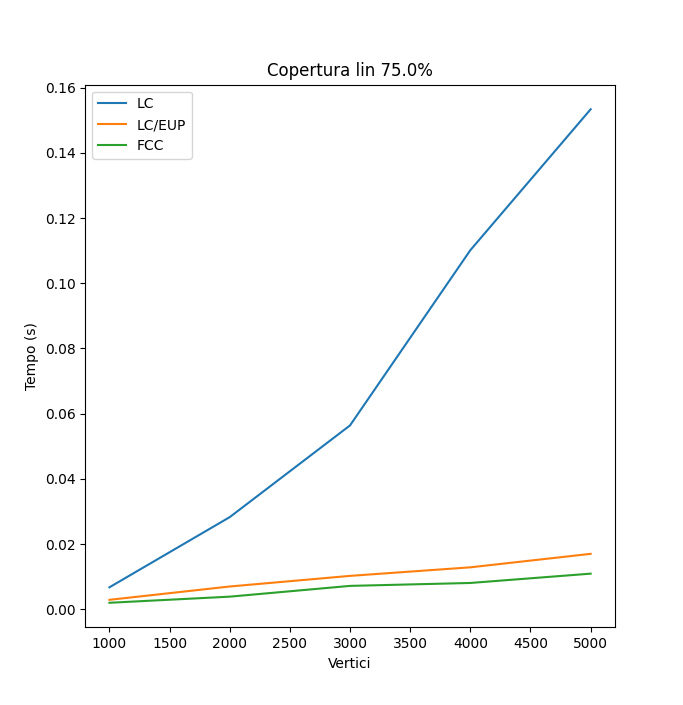
\includegraphics[width=\textwidth]{tests_results/lin75.png}
            \caption{Grafico dei tempi di esecuzione con copertura lineare al 75\%}
            \label{fig:lin75}
        \end{minipage}\hfill
        \begin{minipage}{0.65\textwidth}
            \centering
            \captionsetup{justification=centering}
            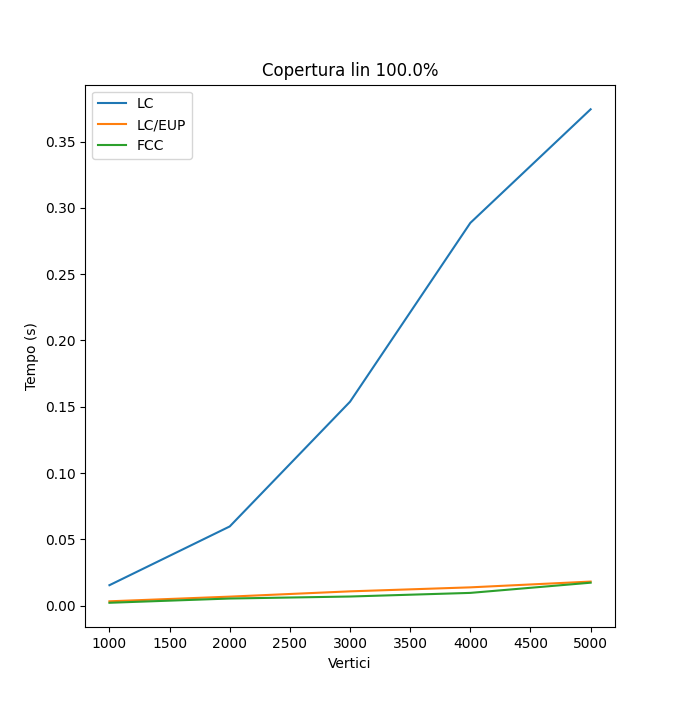
\includegraphics[width=\textwidth]{tests_results/lin100.png}
            \caption{Grafico dei tempi di esecuzione con copertura lineare al 100\%}
            \label{fig:lin100}
        \end{minipage}
    \end{adjustbox}
\end{figure}
\newpage

\subsection{Analisi coperture quadratiche}
Con le coperture quadratiche ci riferiamo ai casi in cui il numero di connessioni è quadratico con il numero di vertici, come riportato in \eqref{quadraticCoverage}.

Analizzando i grafici dei tempi in figura \ref{fig:poly75} e \ref{fig:poly100} possiamo stabilire che:
\begin{enumerate}
    \item \texttt{LC}: continua a comportarsi come nel caso delle coperture lineari come previsto in \eqref{WorstLLCost}, e quindi assume una forma quadratica
          in entrambe le figure e quindi in entrambi i valori di copertura;
    \item \texttt{LC/EUP}: è la curva più bassa di tutte e quindi mostra che nel caso di copertura quadratica l'implementazione con liste concatenate e euristica dell'unione
          pesata è quella che si comporta meglio; nella figura \ref{fig:poly100} la curva si avvicina alla curva \texttt{LC} e questo
          torna col fatto che le due implementazioni condividono lo stesso costo secondo \eqref{WorstLLCost} e \eqref{quadraticWUH};
    \item \texttt{FCC}: è la curva che si comporta in maniera peggiore rispetto alle altre in entrambi i valori di copertura ed è giustificabile secondo
          \eqref{quadraticFPC}.
\end{enumerate}

\begin{table}[!h]
    \parbox{.48\linewidth}{
        \begin{tabular}{|c|c|c|c|}
            \hline
            Vertici & LC    & LC/EUP & FCC   \\ \hline
            100     & 0.001 & 0.001  & 0.003 \\ \hline
            200     & 0.005 & 0.004  & 0.009 \\ \hline
            300     & 0.011 & 0.009  & 0.015 \\ \hline
            400     & 0.021 & 0.017  & 0.024 \\ \hline
            500     & 0.034 & 0.027  & 0.039 \\ \hline
            600     & 0.053 & 0.041  & 0.057 \\ \hline
            700     & 0.074 & 0.058  & 0.081 \\ \hline
            800     & 0.094 & 0.085  & 0.108 \\ \hline
            900     & 0.118 & 0.098  & 0.137 \\ \hline
            1000    & 0.146 & 0.124  & 0.17  \\ \hline
        \end{tabular}
        \centering
        \captionsetup{justification=centering}
        \caption{Mediane dei tempi (s) per una copertura quadratica al 75\%}
    }
    \hfill
    \parbox{.48\linewidth}{
        \centering
        \captionsetup{justification=centering}
        \begin{tabular}{|c|c|c|c|}
            \hline
            Vertici & LC    & LC/EUP & FCC   \\ \hline
            100     & 0.002 & 0.001  & 0.002 \\ \hline
            200     & 0.006 & 0.005  & 0.008 \\ \hline
            300     & 0.013 & 0.012  & 0.018 \\ \hline
            400     & 0.025 & 0.021  & 0.032 \\ \hline
            500     & 0.041 & 0.034  & 0.049 \\ \hline
            600     & 0.058 & 0.049  & 0.07  \\ \hline
            700     & 0.079 & 0.068  & 0.096 \\ \hline
            800     & 0.108 & 0.09   & 0.128 \\ \hline
            900     & 0.137 & 0.115  & 0.167 \\ \hline
            1000    & 0.178 & 0.147  & 0.207 \\ \hline
        \end{tabular}
        \caption{Mediane dei tempi (s) per una copertura quadratica al 100\%}
    }
\end{table}

\begin{figure}[!h]
    \begin{adjustbox}{center}
        \begin{minipage}{0.65\textwidth}
            \centering
            \captionsetup{justification=centering}
            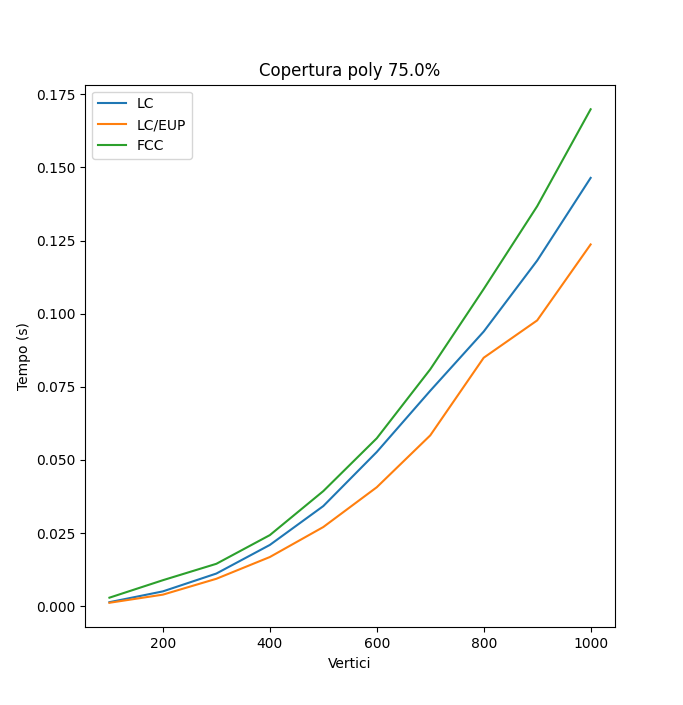
\includegraphics[width=\textwidth]{tests_results/poly75.png}
            \caption{Grafico dei tempi di esecuzione con copertura quadratica al 75\%}
            \label{fig:poly75}
        \end{minipage}\hfill
        \begin{minipage}{0.65\textwidth}
            \centering
            \captionsetup{justification=centering}
            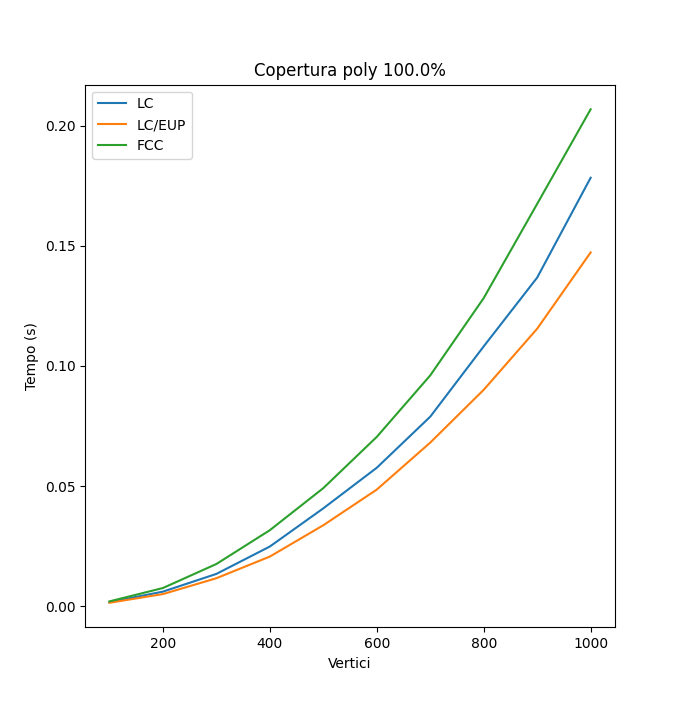
\includegraphics[width=\textwidth]{tests_results/poly100.png}
            \caption{Grafico dei tempi di esecuzione con copertura quadratica al 100\%}
            \label{fig:poly100}
        \end{minipage}
    \end{adjustbox}
\end{figure}
\newpage

\subsection{Considerazioni finali}

Alla luce dei risultati dei test possiamo concludere che le tre implementazioni hanno comportamenti differenti
e incidono notevolmente nella ricerca di componenti connesse. In particolare:

\begin{itemize}
    \item L'implementazione con liste concatenate (senza euristiche) \texttt{LC} è quella che si comporta in modo peggiore
          rispetto alle altre in qualsiasi caso, sia quando il numero di connessioni nel grafo è lineare sia quando è quadratico
          rispetto al numero di vertici presenti;
    \item L'implementazione con foreste di nodi con compressione dei cammini \texttt{FCC} è la migliore nel caso di un numero
          di connessioni lineare rispetto al numero dei vertici, ma quando questi diventano quadratici anche l'implementazione risente
          di questo aumento e tende a comportarsi in maniera peggiore rispetto a tutte le altre implementazioni; solitamente questo tipo
          di implementazione viene accompagnata da un'ulteriore euristica nota come \textit{union by rank} che, insieme alla compressione
          dei cammini, tende ad avere costi computazionali migliori in tutti i casi, ma in questa analisi è stata richiesta l'implementazione
          della semplice compressione dei cammini;
    \item L'implementazione con liste concatenate attraverso l'euristica dell'unione pesata, nei casi analizzati, è quella che si comporta
          complessivamente in maniera migliore, quindi considerando sia il caso di numero di connessioni lineare, sia il caso quadratico,
          rispetto ai vertici; ad ogni modo non è detto che non si possano trovare implementazioni più veloci di questa, e un esempio è la
          \textit{union by rank} citata nel punto precedente.
\end{itemize}

